\chapter{Fundamentação Teórica}
% feature extraction in medical images + complex networks + recurrent neural networks gerando embedding topológico + hybrid models gerando embedding visual + late fusion via mlp

\section{Extração de \textit{Features}}
\label{sec:extracao-features}

Em reconhecimento de padrões, uma \textit{feature} é uma medida numérica que resume aspectos relevantes da imagem, como bordas, texturas, formas e padrões de cor. A extração de \textit{features} é o processo que mapeia a imagem bruta para uma representação de menor dimensão, utilizável, por exemplo, para melhorar a classificação por modelos de \textit{deep learning} \cite{ramossoto2025miafex}. Em imagens médicas, uma \textit{feature} corresponde a uma característica ou padrão relevante para a tarefa diagnóstica, como forma, tamanho, textura, densidade ou intensidade das estruturas observadas \cite{dehbozorgi2025}. A qualidade dessa representação influencia a capacidade de generalização do classificador, principalmente quando há poucos dados, cenário recorrente na área da saúde devido a protocolos de privacidade, custos de aquisição e necessidade de especialistas para a rotulação \cite{litjens2017survey}. Nenhum método de extração é superior em todos os casos, e a escolha depende da disponibilidade e da dimensionalidade dos dados, da existência de rótulos e da estratégia de aprendizado \cite{ahmed2023review}.

\subsection{Descritores clássicos (\textit{handcrafted})}
\label{subsec:features-classicas}

Os descritores clássicos (\textit{handcrafted}) são calculados por procedimentos matemáticos fixados previamente, sem aprendizado a partir dos dados. Entre os mais utilizados em imagens médicas estão as estatísticas de primeira ordem, a matriz de coocorrência de níveis de cinza (GLCM), os padrões binários locais (LBP), o histograma de gradientes orientados (HOG), os filtros de Gabor e a transformada de características invariantes à escala (SIFT) \cite{ramossoto2025miafex,ahmed2023review}. Três deles (GLCM, LBP e HOG) são adotados neste trabalho como métodos comparativos da técnica proposta, e aparecem juntos em estudos de classificação de imagens médicas \cite{dehbozorgi2025,ramossoto2025miafex}.


\citeonline{haralick1973textural} propuseram caracterizar a textura de um bloco de imagem por matrizes de dependência de tons de cinza, hoje conhecidas como GLCM. Cada elemento $(i,j)$ da matriz registra quantas vezes um pixel de tom $i$ ocorre como vizinho de um pixel de tom $j$, dada uma distância $d$ e uma direção angular (0°, 45°, 90° ou 135°). A partir da matriz normalizada, os autores definiram 14 medidas de textura, entre elas o contraste, a correlação, a variância e a entropia, e aplicaram essas características como entradas em classificadores que obtiveram acurácias de teste acima de 82\% em fotomicrografias de arenitos, fotografias aéreas e imagens de satélite. Como limitações, \citeonline{he1989texture} apontam que a matriz depende da variação regional do fundo de intensidade da imagem e que a escolha do vetor de deslocamento é problemática.

O espectro de textura, proposto por \citeonline{he1989texture} a partir do conceito de unidade de textura, codifica cada um dos oito vizinhos de um pixel central em um de três valores (0, 1 ou 2), conforme sua relação de intensidade com o pixel central, o que resulta em $3^8 = 6561$ unidades de textura possíveis. A distribuição de frequência dessas unidades ao longo da imagem funciona como descritor, e a redução das intensidades a três valores diminui o custo de cálculo e elimina a influência do fundo regional de intensidade e do ruído \cite{wang1990texture}. Em quatro texturas naturais do álbum de Brodatz, o espectro alcançou acurácia média de 97,5\% com um classificador de distância mínima \cite{wang1990texture}. Os LBP seguem a mesma ideia de codificar a relação entre o pixel central e seus vizinhos, com uma codificação binária mais compacta e a descrição da imagem pelo histograma dos códigos. % TODO: citar Ojala et al. (1996; 2002) para a formulação binária do LBP, pois os PDFs fornecidos descrevem o espectro de textura (antecessor), não o LBP em si.

O HOG foi proposto por \citeonline{dalal2005histograms} para detecção de pessoas e descreve a imagem pela distribuição local das direções de gradiente. A janela é dividida em células, em cada uma é acumulado um histograma das orientações de gradiente ponderadas pela magnitude, e as respostas são normalizadas quanto ao contraste em blocos sobrepostos para ganhar invariância a iluminação. A concatenação dos histogramas forma o descritor, que alimentou uma máquina de vetores de suporte (SVM) linear e reduziu as taxas de falsos positivos em mais de uma ordem de magnitude em relação ao melhor detector baseado em \textit{wavelets} de Haar \cite{dalal2005histograms}. Apesar de concebido para detecção, o HOG é empregado como descritor de bordas e forma em imagens médicas \cite{ramossoto2025miafex}.

\subsection{Extração por aprendizado profundo}
\label{subsec:features-profundas}

Os descritores \textit{handcrafted} capturam relações locais entre pixels, em escalas e vizinhanças definidas previamente. As redes neurais convolucionais (CNNs), em contraste, aprendem filtros que vão de bordas e texturas nas primeiras camadas até padrões semânticos nas camadas finais, e se tornaram uma abordagem consolidada em análise de imagens médicas \cite{litjens2017survey}. Em domínios com poucos dados, a transferência de aprendizado (\textit{transfer learning}) permite empregar uma rede pré-treinada em uma base grande, como a ImageNet, como extrator de \textit{features}, e a ativação de uma camada intermediária ou final é utilizada como vetor de características. Em \citeonline{dehbozorgi2025}, cinco redes pré-treinadas (VGG16, ResNet50, DenseNet121, MobileNetV2 e InceptionV3) em geral superaram os métodos estatísticos e de \textit{radiomics} em sensibilidade e em tempo de extração, e a DenseNet121 alcançou 98,6\% na base de tomografia de coerência óptica, contra 91\% do \textit{radiomics}. Os autores apontam como limitações a necessidade de GPUs, a dependência de grandes bases de dados e a baixa interpretabilidade.

A necessidade de capturar dependências de longo alcance motivou o uso de \textit{Vision Transformers} (ViT) \cite{dosovitskiy2020image} e de arquiteturas híbridas que combinam convolução e atenção, como a CoAtNet \cite{dai2021coatnet}, discutidas em revisões sobre \textit{transformers} em imagens médicas \cite{shamshad2023transformers}. CNNs e ViTs tendem ao sobreajuste quando treinados em bases pequenas ou com alta variância intraclasse, e o MIAFEx \cite{ramossoto2025miafex} refina o \textit{token} de classificação de um \textit{Transformer} por pesos aprendíveis para atenuar esse problema. Em bases médicas pequenas, o MIAFEx superou extratores clássicos, CNNs e ViTs, e os autores reportam que essa vantagem diminui à medida que o conjunto de dados cresce. Como lesões e estruturas de interesse variam em tamanho e aparência, também é recorrente a análise em várias escalas, como na MMS-Net \cite{zhao2023mmsnet}, que combinou contexto multiescala local e global e manteve resultados competitivos com apenas 20\% dos dados de treino. A análise da imagem em vários níveis de vizinhança é análoga à variação progressiva do raio de conexão nas redes complexas (Seção~\ref{sec:redes-complexas}). \textit{Features} aprendidas sobre dados ordenados por redes recorrentes e features topológicas extraídas de redes complexas são tratadas nas Seções~\ref{sec:rnn-topologicas} e \ref{sec:redes-complexas},

\section{Redes Complexas}
\label{sec:redes-complexas}

A teoria de Redes Complexas (CN, do inglês \textit{Complex Networks}) é uma abstração para modelar sistemas naturais cujos elementos interagem de maneira não trivial \cite{BOCCALETTI2006175}. Essas redes foram empregadas para modelar os pixels de uma imagem e suas relações de vizinhança, o que permite que descritores baseados em topologia quantifiquem propriedades de textura de forma discriminativa \cite{BACKES2013168, ribas2020fusion, ribas2024colorspectral}. Neste trabalho, a abordagem segue a transformação por redes complexas empregada em \citeonline{CNT} e é aplicada a imagens histopatológicas.

\subsection{Modelagem da imagem como rede direcionada}
\label{subsec:cn-modelagem}

Cada imagem é representada como uma rede complexa direcionada e ponderada $G = (V, E)$, na qual cada pixel é modelado como um vértice e as conexões entre pixels são estabelecidas dentro de um raio máximo $r_{max}$. Para um pixel $i = (x_i, y_i)$ em um canal de cor $c$ da imagem $I$, é definido um vértice $v_i^{(c)} \in V$. Uma aresta direcionada é criada entre os vértices $v_i^{(c)}$ e $v_j^{(c_w)}$ quando a distância euclidiana quadrática entre os pixels satisfaz a Equação~\ref{eq:cn-aresta}:
\begin{equation}
\rho_{ij}^2 = (x_i - x_j)^2 + (y_i - y_j)^2, \qquad 0 < \rho_{ij}^2 \leq r_{max}^2,
\label{eq:cn-aresta}
\end{equation}
em que $x$ e $y$ são as coordenadas dos pixels e $\rho_{ij}$ é a distância euclidiana entre eles. A condição $\rho_{ij}^2 > 0$ exclui laços, isto é, a conexão de um pixel consigo mesmo. Cada aresta é associada a um raio discreto $r \in \{1, 2, \ldots, r_{max}\}$, definido como o menor inteiro que satisfaz $(r-1)^2 < \rho_{ij}^2 \leq r^2$, o que permite acumular as medidas da rede progressivamente sobre vizinhanças cada vez maiores.

O peso atribuído a cada aresta é a diferença absoluta de intensidade entre os pixels conectados, conforme a Equação~\ref{eq:cn-peso}:
\begin{equation}
w_{ij} = \left| I(x_i, y_i, c) - I(x_j, y_j, c_w) \right|.
\label{eq:cn-peso}
\end{equation}
O direcionamento de cada aresta é determinado pelas intensidades relativas dos pixels incidentes e vai do pixel de menor intensidade para o de maior intensidade. Quando $I(x_i, y_i, c) < I(x_j, y_j, c_w)$, a conexão é classificada como de saída (\textit{out}) a partir de $v_i$ e de entrada (\textit{in}) em $v_j$. No caso contrário, ela é classificada como de entrada em $v_i$. Conexões entre pixels de mesma intensidade são contabilizadas em ambas as direções. O grau de saída de um vértice conta seus vizinhos mais claros, e o grau de entrada conta seus vizinhos mais escuros.

\subsection{Medidas topológicas e configurações da rede}
\label{subsec:cn-medidas}

O grau (\textit{degree}) e a força (\textit{force}) são calculados para cada vértice pela acumulação das quantidades correspondentes até o raio $r$, nas versões de saída e de entrada. O grau quantifica o número de conexões dentro da vizinhança considerada, como na Equação~\ref{eq:cn-grau}:
\begin{equation}
d_{out}(v_i, r) = \sum_{k=1}^{r} n_{out}(v_i, k),
\label{eq:cn-grau}
\end{equation}
em que $n_{out}(v_i, k)$ é o número de arestas de saída de $v_i$ cujo raio discreto vale $k$, e o grau de entrada, $d_{in}(v_i, r)$, é calculado de forma análoga a partir de $n_{in}(v_i, k)$. A força incorpora as diferenças de intensidade e a proximidade entre os pixels, o que a torna sensível aos gradientes locais de textura. Para uma rede construída com raio $r$, cada aresta $(v_i, v_j)$ recebe um peso de força que combina a diferença de intensidade normalizada com a distância normalizada, conforme a Equação~\ref{eq:cn-forca-peso}:
\begin{equation}
\omega_{ij}^{(r)} =
\begin{cases}
\dfrac{w_{ij}}{2L}, & r = 1,\\[8pt]
\dfrac{1}{2}\left[\dfrac{w_{ij}}{L} + \dfrac{\rho_{ij}^2-1}{r^2-1}\right], & r \geq 2,
\end{cases}
\label{eq:cn-forca-peso}
\end{equation}
em que $L = 255$ é o nível máximo de intensidade para imagens de 8 bits e $w_{ij}$ é o peso dado pela Equação~\ref{eq:cn-peso}. A força de saída acumulada é dada pela Equação~\ref{eq:cn-forca}:
\begin{equation}
\text{force}_{out}(v_i, r) = \sum_{v_j \in \mathcal{N}_{out}^{(r)}(v_i)} \omega_{ij}^{(r)},
\label{eq:cn-forca}
\end{equation}
em que $\mathcal{N}_{out}^{(r)}(v_i)$ é o conjunto de vértices conectados a $v_i$ por arestas de saída com $\rho_{ij}^2 \leq r^2$, e $\text{force}_{in}$ é definida de forma análoga sobre as arestas de entrada. O fator $r^2 - 1$ na Equação~\ref{eq:cn-forca-peso} é o valor máximo de $\rho_{ij}^2 - 1$ dentro de uma vizinhança de raio $r$, o que mantém o termo de distância no intervalo $[0, 1]$. Para $r = 1$, a única distância quadrática possível é $\rho_{ij}^2 = 1$, de modo que o termo de distância é nulo e o fator $r^2 - 1$ anularia o denominador, e nesse caso o peso é reduzido à componente de intensidade. As medidas resultam em quatro grandezas por vértice: grau de saída, grau de entrada, força de saída e força de entrada.

Para estender as medidas aos três canais de cor das imagens histopatológicas RGB, as formulações anteriores podem ser aplicadas em três configurações de rede \cite{Scabini_2020}: \textit{within-channel}, com $c = c_w$, \textit{between-channel}, com $c \neq c_w$, e \textit{full}, que inclui simultaneamente conexões intracanal e intercanal. A configuração \textit{full} é adotada neste trabalho para capturar conjuntamente as transições de intensidade e as relações cromáticas entre canais \cite{CNT}. O raio máximo $r_{max}$ foi selecionado pela avaliação de raios de 1 a 15 em todas as bases de dados, esse intervalo foi selecionado considerando valores explorados na literatura \cite{CNT, SCABINI2026}. A entropia de Shannon, utilizada para quantificar as mudanças na distribuição dos valores topológicos, cresceu até aproximadamente $r = 10$ e atingiu um platô a partir daí, e a entropia amostral teve pico em $r = 10$ e decresceu depois, conforme mostra a Figura \ref{fig:entropia-todos-e-media}. Esses resultados, somados a achados anteriores de que combinações multiescala de raios são úteis \cite{ribas2024colorspectral, CNT}, justificam a adoção de $r_{max} = 10$. À medida que $r$ cresce, as características locais dos menores raios dão lugar a características progressivamente mais globais, e essa evolução ao longo dos raios forma a sequência processada pela via recorrente (Seção~\ref{sec:rnn-topologicas}).

\begin{figure}
	\begin{center}
		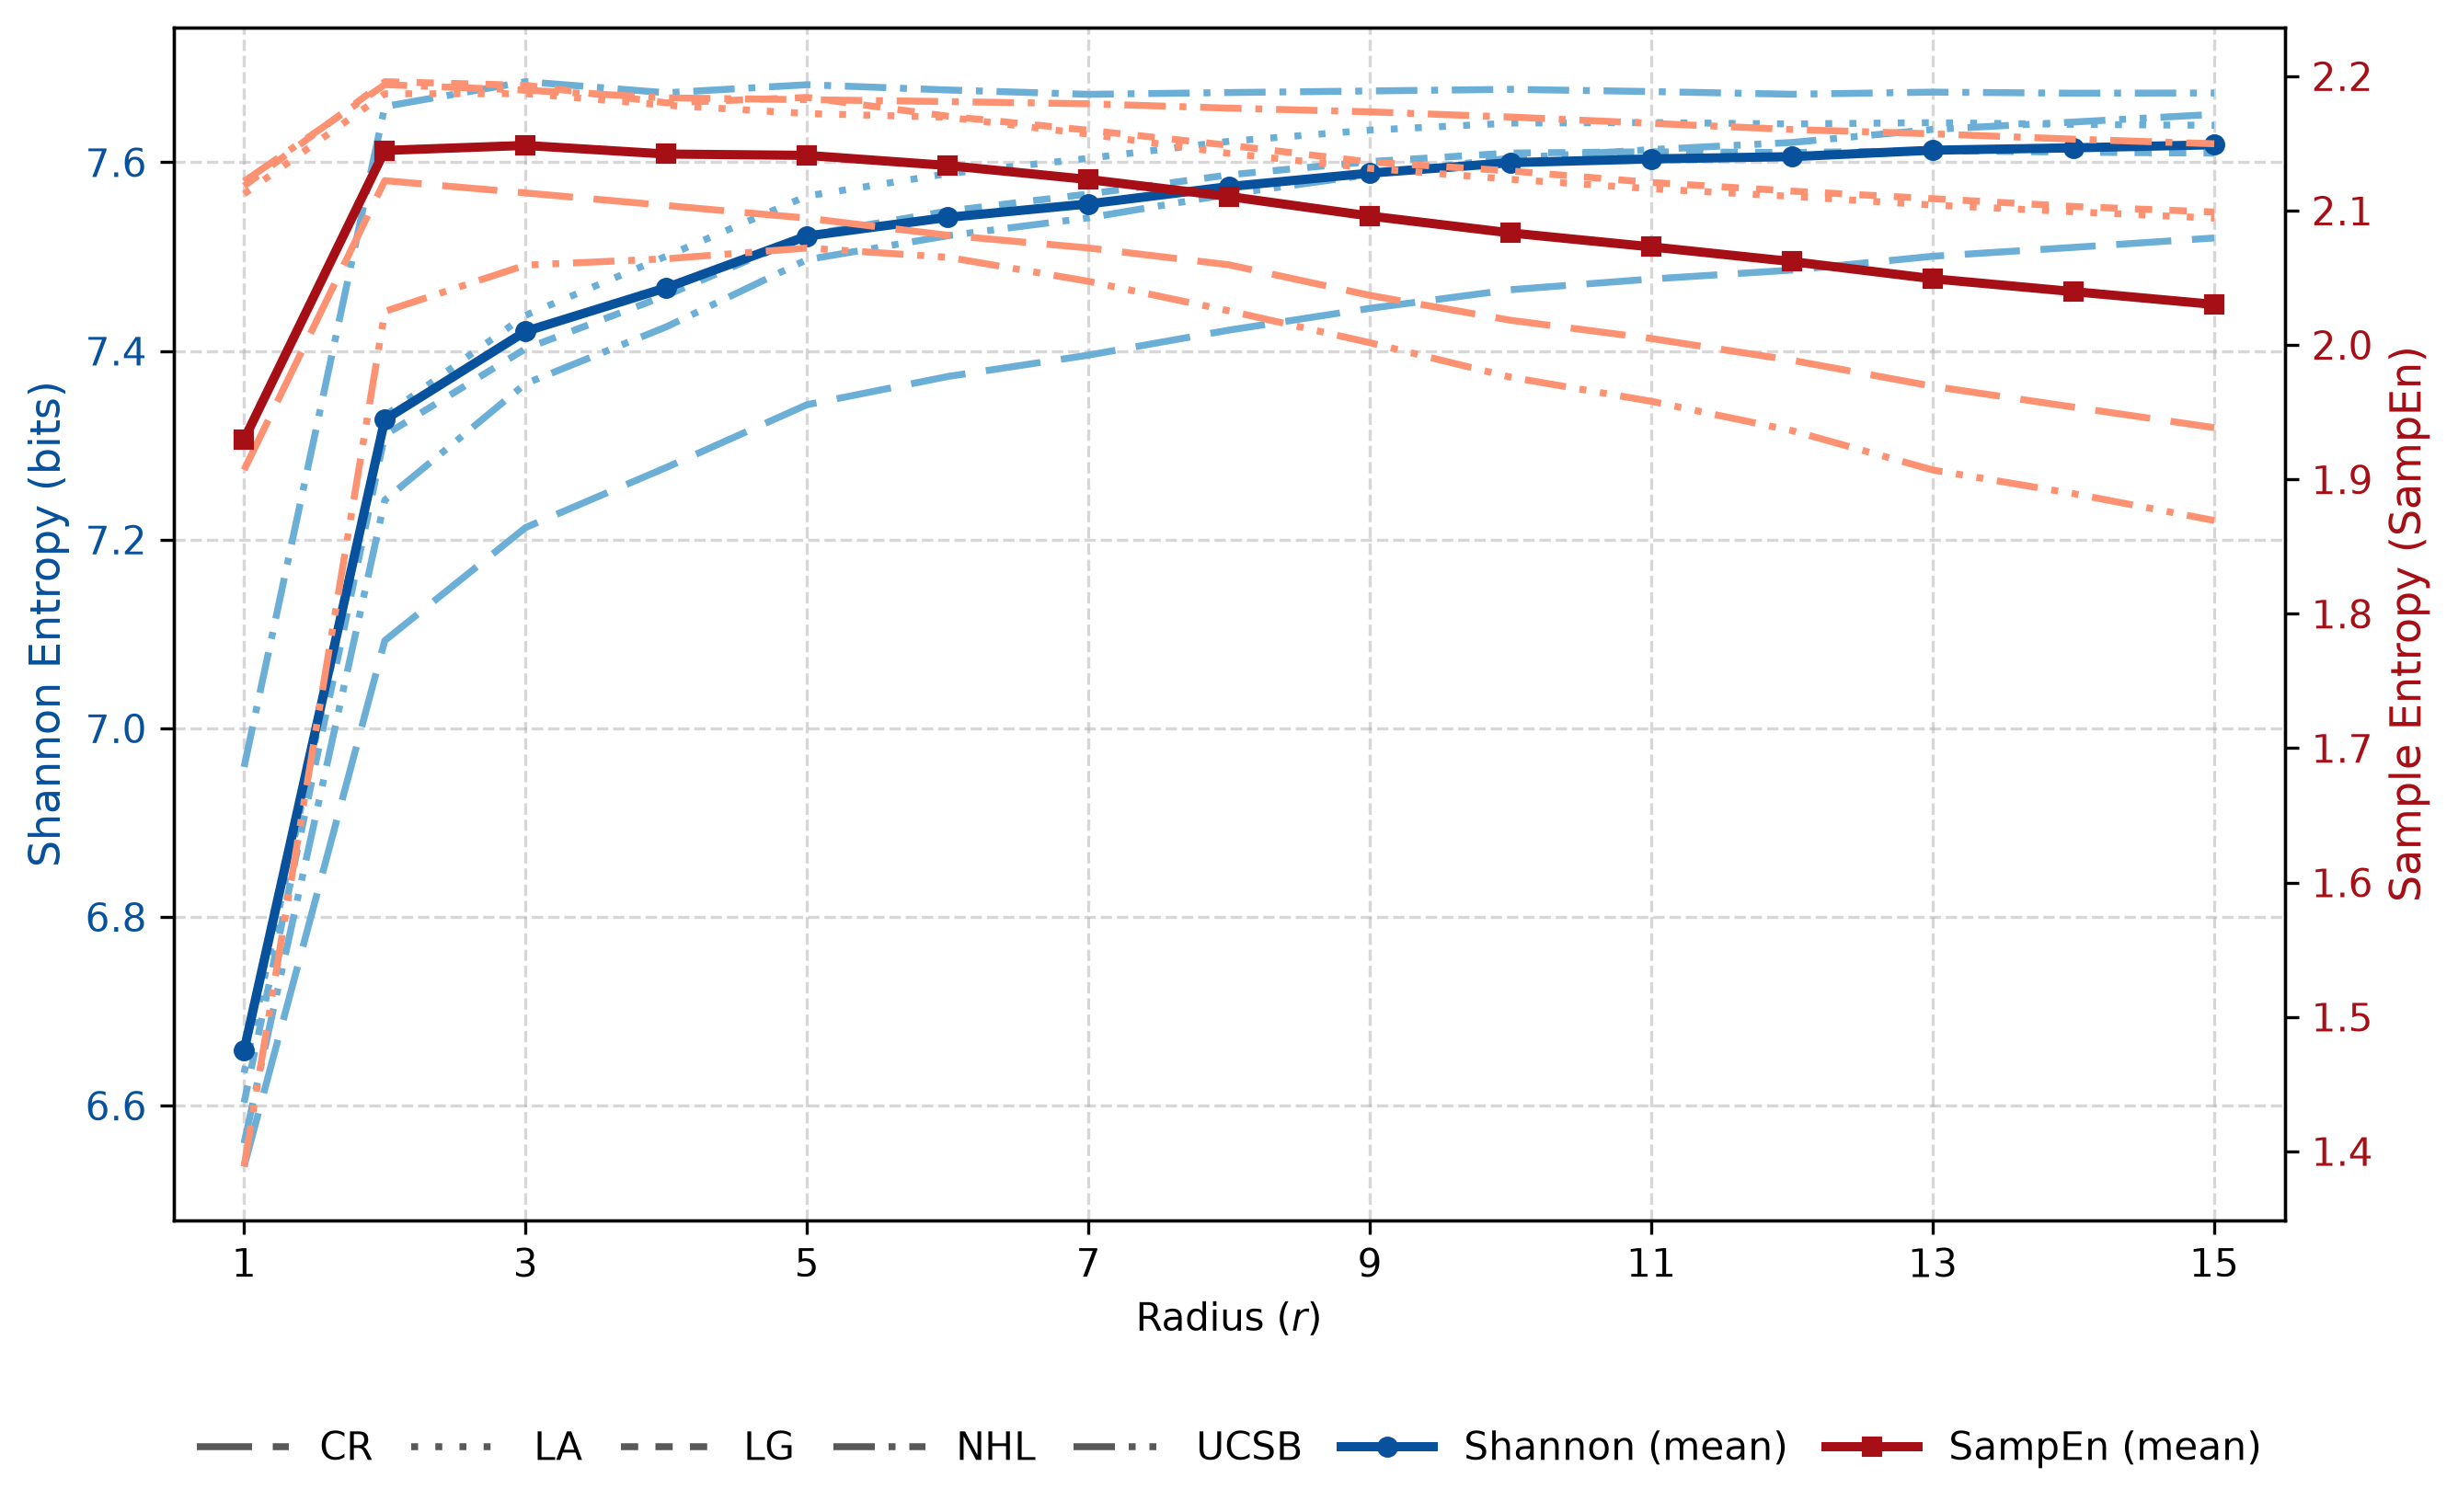
\includegraphics[width=0.95\textwidth]{img/entropia_todos_e_media.png}
	\end{center}
	\caption{Entropias de Shannon e amostral em função do raio de conexão (1 a 15) para as bases CR, LA, LG, NHL e UCSB. As linhas tracejadas correspondem a cada base e as linhas contínuas, à média entre as bases.}
	\label{fig:entropia-todos-e-media}
\end{figure}


\section{RNN na Extração de \textit{Features} Topológicas}
\label{sec:rnn-topologicas}

Na arquitetura proposta, a via sequencial transforma a evolução topológica da imagem, modelada como rede complexa (Seção~\ref{sec:redes-complexas}), em um \textit{embedding} topológico que é combinado com o \textit{embedding} visual no estágio de fusão tardia (Seção~\ref{sec:fusao-tardia}). A \textit{Spatio-Spectral Network} depende de um conjunto de raios \cite{Scabini_2020}, e \citeonline{ribas2024colorspectral} exploraram essa dimensão: as medidas topológicas de cada vértice (grau de saída, força de entrada e força de saída) foram calculadas em vários raios $r = \{1, 2, \ldots, R\}$, e os valores obtidos em $r = 1, \ldots, R-1$ formaram um vetor de entrada usado para prever o valor da mesma medida no raio máximo $R$. Os autores descrevem esse procedimento como uma análise multiescala da evolução topológica dos vértices, e a maior acurácia média nos três conjuntos de textura colorida foi obtida pela combinação de duas representações, com $R = 4$ e $R = 10$, o que indica que tanto a escala local quanto as escalas mais amplas contribuem para a discriminação.

A proposta deste trabalho difere no tratamento da sequência, onde em \citeonline{ribas2024colorspectral}, a sequência de raios é achatada em um único vetor de entrada de uma rede neural aleatorizada de uma camada oculta, e o descritor da imagem são os pesos da camada de saída, calculados por mínimos quadrados regularizados. O artigo utiliza a sigla RNN para essa rede, mas ela não é recorrente, pois os valores de cada raio entram simultaneamente e a arquitetura não explora a ordem entre eles. Neste trabalho, a sequência é tratada como tal: uma série de passos $x_1, x_2, \ldots, x_R$ é definida, em que $x_t \in \mathbb{R}^{d}$ reúne as medidas topológicas calculadas sobre o grafo construído com o raio $r_t$, e uma rede recorrente a lê passo a passo, do menor raio para o maior. Essa organização reflete a hipótese de que as macroestruturas da imagem dependem da organização das microestruturas, de modo que o descritor do raio $r_t$ deve ser interpretado à luz do que foi observado nos raios anteriores.
% TODO: definir como o vetor x_t é obtido a partir das medidas de vértice (por exemplo, média, desvio padrão e histograma de cada uma das quatro medidas, na rede \textit{Full}, conforme a Seção~\ref{sec:redes-complexas}), o número de raios R e a dimensão d

\subsection{Redes recorrentes e \textit{embedding} topológico}
\label{subsec:rnn-fundamentos}

Uma rede neural recorrente processa uma sequência um elemento por vez e mantém um estado interno que carrega informação sobre os elementos anteriores \cite{lecun2015deep}. Na rede recorrente simples de \citeonline{elman1990finding}, o estado oculto depende da entrada atual e do estado anterior, com parâmetros compartilhados por todos os passos, e o número de parâmetros não depende do comprimento da sequência. O treinamento por retropropagação enfrenta o desaparecimento ou a explosão dos gradientes à medida que o intervalo entre entrada e saída aumenta \cite{bengio1994learning}, e a LSTM \cite{hochreiter1997long} mitiga esse problema com uma célula de memória $c_t$ controlada por portas. Na formulação usual, que inclui a porta de esquecimento \cite{gers2000learning}, as atualizações são:
\begin{align}
f_t &= \sigma\!\left(W_f x_t + U_f h_{t-1} + b_f\right), \label{eq:lstm-f}\\
i_t &= \sigma\!\left(W_i x_t + U_i h_{t-1} + b_i\right), \label{eq:lstm-i}\\
o_t &= \sigma\!\left(W_o x_t + U_o h_{t-1} + b_o\right), \label{eq:lstm-o}\\
\tilde{c}_t &= \tanh\!\left(W_c x_t + U_c h_{t-1} + b_c\right), \label{eq:lstm-ctil}\\
c_t &= f_t \odot c_{t-1} + i_t \odot \tilde{c}_t, \label{eq:lstm-c}\\
h_t &= o_t \odot \tanh(c_t), \label{eq:lstm-h}
\end{align}
em que $\sigma$ é a função sigmoide, $\odot$ denota o produto elemento a elemento e $f_t$, $i_t$ e $o_t$ são as portas de esquecimento, entrada e saída. A GRU \cite{cho2014learning} é uma alternativa com menos portas e menos parâmetros, e \citeonline{greff2017lstm} concluíram, em cerca de 5.400 execuções de treinamento sobre oito variantes da LSTM, que nenhuma melhorou significativamente a LSTM padrão, o que sustenta seu uso como ponto de partida.

Uma RNN unidirecional lê a sequência em um único sentido, e a RNN bidirecional \cite{schuster1997bidirectional} utiliza duas redes independentes, uma lendo a sequência na ordem original e outra na ordem inversa, e combina seus estados:
\begin{equation}
h_t = \left[\overrightarrow{h}_t \,\Vert\, \overleftarrow{h}_t\right].
\label{eq:bilstm}
\end{equation}
Em classificação de fonemas por quadro, as redes bidirecionais superaram as unidirecionais e a LSTM superou as RNNs convencionais \cite{graves2005framewise}. No presente caso, a sequência de raios está integralmente disponível na inferência, e não há restrição de causalidade que impeça a leitura nos dois sentidos. Como a imagem inteira recebe um único rótulo, a rede opera no formato \textit{many-to-one}, e o \textit{embedding} topológico $z_{\mathrm{top}}$ é definido como o estado final: $z_{\mathrm{top}} = h_R$ em uma rede unidirecional e, em uma rede bidirecional, $z_{\mathrm{top}} = [\overrightarrow{h}_R \,\Vert\, \overleftarrow{h}_1]$. Esse vetor tem dimensão fixa, o que permite concatená-lo ao \textit{embedding} visual (Seção~\ref{sec:rede-hibrida}) e entregá-lo ao classificador da fusão tardia. Diferentemente do descritor de \citeonline{ribas2024colorspectral}, cujos pesos de saída são obtidos por mínimos quadrados sem retropropagação, os parâmetros da rede recorrente são aprendidos por gradiente a partir do rótulo da classe, e o \textit{embedding} é otimizado para a classificação.
% TODO: definir o tipo de célula (LSTM, GRU ou BiLSTM), o número de camadas, a dimensão do estado oculto e a forma de treinamento da via sequencial (conjunta com a fusão ou separada)

\subsection{Redes recorrentes sobre \textit{features} de imagens e escolha da arquitetura}
\label{subsec:rnn-literatura}

Embora a recorrência seja associada a sequências temporais, diversos trabalhos a aplicaram a \textit{features} extraídas de imagens médicas, tratando-as como uma sequência ordenada. \citeonline{shalini2026saclstm} organizaram \textit{features} de imagens de histopatologia de mama em sequência para que a LSTM capture relações entre seus elementos que uma CNN, centrada em padrões locais, pode não explorar, e reportaram acurácia de 99,31\% na base BreakHis. \citeonline{mathiyalagi2026hclstm} alimentaram uma CNN-LSTM com \textit{features} de textura da GLCM reduzidas por análise de componentes principais, em tomografias de pulmão, com acurácia de 98,45\% e sem validação externa, e \citeonline{akanksha2022leukemia} utilizaram \textit{features} SIFT como entrada de uma RNN para classificar leucemia. Em outros casos, a sequência é formada por mapas de uma CNN, como em \citeonline{zeng2025mssfn}, em que uma BiLSTM modelou a relação entre fatias de tomografias de pulmão e sua remoção reduziu a acurácia em 12,42\% na ablação. Fora de imagens, \citeonline{lin2022mslstm} mostraram que diferentes comprimentos de sequência de entrada de uma LSTM contêm informações distintas e afetam a acurácia, o que é análogo à escolha do conjunto de raios $r$, e \citeonline{kang2024mmdb} integraram, por uma camada totalmente conectada, um ramo de convoluções dilatadas multiescala com BiLSTM e um ramo sobre informação de estrutura molecular, uma organização de dupla via semelhante à do modelo aqui proposto.

A maior parte dos resultados acima de 98\% provém de conjuntos pequenos, de dados tabulares ou de protocolos com validação limitada, e constitui evidência de viabilidade e não de superioridade. Nenhum desses trabalhos constrói a sequência a partir de descritores topológicos de um grafo em raios crescentes, e a contribuição aqui proposta é essa organização, apoiada na formulação de \citeonline{ribas2024colorspectral}. Quanto à escolha da rede recorrente, a literatura consultada não traz comparação direta entre arquiteturas para sequências de descritores topológicos, e os argumentos são de plausibilidade. Um perceptron multicamadas sobre o vetor achatado dos $R$ passos trata todas as posições como entradas independentes, enquanto a rede recorrente acumula em seu estado o que foi visto nos raios anteriores. Os \textit{transformers} requerem poucas premissas de projeto sobre a estrutura dos dados \cite{khan2022transformers} e dependem de grandes volumes de dados ou de pré-treinamento \cite{dosovitskiy2020image}, e a via sequencial não dispõe de modelo pré-treinado para descritores topológicos, com bases médicas de dezenas a poucas centenas de imagens e conjuntos de raios curtos (valores de $R$ entre 4 e 12 em \citeonline{ribas2024colorspectral}). \citeonline{fawaz2019deep} observam, em revisão de arquiteturas profundas para classificação de séries temporais, que as redes recorrentes raramente são usadas por serem projetadas para uma saída por instante, sofrerem com gradientes em séries longas e serem difíceis de paralelizar. Os dois primeiros motivos são atenuados neste trabalho, pois a rede opera no formato \textit{many-to-one} e a sequência é curta, e a mesma revisão trata perceptrons multicamadas e CNNs como alternativas legítimas. A vantagem da recorrência permanece uma hipótese a ser verificada experimentalmente, por exemplo contra um perceptron multicamadas sobre o vetor achatado e uma CNN unidimensional sobre a sequência.
% TODO: se a banca exigir, transformar essa comparação em um estudo de ablação do capítulo de experimentos

\section{Redes Híbridas para Extração de \textit{Features} Visuais}
\label{sec:rede-hibrida}

Na arquitetura proposta, a via visual extrai, diretamente da imagem RGB, o \textit{embedding} visual que é combinado com o \textit{embedding} topológico no estágio de fusão (Seção~\ref{sec:fusao-tardia}). As CNNs extraem com eficiência padrões locais, como bordas, texturas e pequenas estruturas, mas o campo receptivo restrito das convoluções dificulta a captura de contexto global e de dependências de longo alcance \cite{ma2026cihm}. Os \textit{Vision Transformers} (ViT) \cite{dosovitskiy2020image} abordam esse problema pela autoatenção sobre sequências de \textit{patches}, e são estudados em imagens médicas \cite{shamshad2023transformers}, mas a autoatenção tem custo computacional quadrático em relação ao tamanho da imagem \cite{ma2026cihm}, e os \textit{transformers} tradicionais têm dificuldade em representar o contexto local \cite{garbaz2025gsac}. As arquiteturas híbridas combinam a captura de padrões locais das CNNs com a modelagem global dos \textit{transformers}, em geral com blocos convolucionais que extraem informação localizada e mecanismos de atenção que integram o contexto global, o que é relevante em patologia computacional, em que a interpretação depende de detalhes morfológicos finos e de padrões em escala de tecido \cite{oliveira2025hybrid}.

\subsection{Estratégias de integração entre convolução e atenção}
\label{subsec:hibrida-estrategias}

A literatura descreve diversas formas de integrar CNNs e \textit{transformers}, e \citeonline{oliveira2025hybrid} resumem duas taxonomias existentes, atribuídas a Kim et al. e a Khan et al. A taxonomia de Kim et al. separa projetos paralelos, em que CNN e ViT operam de forma independente e têm suas saídas fundidas, por exemplo por atenção cruzada, de projetos sequenciais, em que as \textit{features} de um módulo alimentam o outro. A de Khan et al. é mais granular e distingue a integração em camadas iniciais, em camadas laterais, sequencial, paralela, em bloco, hierárquica, baseada em atenção e por reforço de canais. Os próprios autores propõem uma taxonomia por tarefa, na qual as arquiteturas de classificação consistem em um codificador de \textit{features}, um estágio de adaptação e um classificador final, organização que corresponde, neste trabalho, ao MobileViT como codificador e ao perceptron multicamadas (MLP) da fusão tardia como classificador. A rede proposta é um projeto paralelo, pois as vias visual e topológica operam de forma independente e são combinadas apenas na fusão tardia. Na revisão de escopo de \citeonline{oliveira2025hybrid}, que analisou 39 estudos de histopatologia, a maioria dos trabalhos adotou arquiteturas integradas ou sequenciais, e os autores apontam limitações recorrentes: poucos estudos realizaram validação externa, muitos utilizaram bases pequenas e homogêneas, a maioria empregou validação por \textit{holdout} em vez de validação cruzada e apenas 35,9\% utilizaram técnicas de explicabilidade. O delineamento experimental deste trabalho considera essas observações e prevê validação cruzada estratificada e comparação com modelos de via única.

\subsection{MobileViT: o extrator adotado}
\label{subsec:hibrida-mobilevit}

A CoAtNet \cite{dai2021coatnet} empilha convoluções eficientes nos estágios iniciais, que operam sobre mapas de alta resolução, e blocos de autoatenção nos estágios finais, sobre mapas de baixa resolução \cite{zaidkilani2024dualstream}, e ilustra o princípio de combinar convolução e atenção em sequência. O extrator adotado neste trabalho é o MobileViT, proposto por \citeonline{mehta2022mobilevit} como uma rede híbrida leve. No bloco MobileViT, uma convolução $n\times n$ seguida de uma convolução pontual $1\times1$ gera uma representação local do tensor de entrada, essa representação é dividida em \textit{patches} não sobrepostos, sobre os quais um \textit{Transformer} codifica as relações entre \textit{patches}, e o resultado é reorganizado, concatenado com a entrada e processado por uma nova convolução $n\times n$, que funde as informações local e global \cite{ding2023himvit}. O bloco combina convolução e autoatenção em um mesmo módulo, característica que \citeonline{oliveira2025hybrid} atribuem aos projetos integrados.

A adoção do MobileViT tem três justificativas. A primeira é que o vetor final carrega informação local e global em um único módulo \cite{ding2023himvit}. A segunda é o baixo custo computacional, pois o HI-MViT, derivado do MobileViT, é descrito como leve e implantável em dispositivos móveis \cite{ding2023himvit}, e o MobileViT tem eficiência superior à de \textit{transformers} puros \cite{wang2026msi}, perfil adequado às bases pequenas previstas neste trabalho (de 68 a 528 imagens). A terceira é o desempenho em imagens médicas de diferentes modalidades: o HI-MViT alcançou acurácia de 0,932 e F1 de 0,931 na base ISIC-2018 e superou em 3,4\% a acurácia da ConvNeXt \cite{ding2023himvit}, e, em microscopia multiespectral de tecido, o MobileViT obteve a maior acurácia (91,70\%) entre cinco arquiteturas, incluindo Swin-Transformer e ResNet \cite{wang2026msi}. Outras variações exploram o mesmo princípio, como o LightSE-MobileViT, que insere um bloco \textit{Squeeze-and-Excitation} para classificar câncer oral \cite{kabir2025semobilevit}, e a combinação de ResNet e MobileViT em um modelo de dupla entrada para ultrassom de mama \cite{zou2023dualinput}.

\subsection{Evidências comparativas e \textit{embedding} visual}
\label{subsec:hibrida-evidencias}

Arquiteturas de ramos paralelos também são empregadas. No CIHM, a camada CiMC combina em paralelo um ramo de modelo de espaço de estados (Mamba), que captura dependências de longo alcance com complexidade linear, e um bloco convolucional, que extrai detalhes locais \cite{ma2026cihm}, e o GSAC-UFormer integra em paralelo convolução em grupos e autoatenção adaptada por CNN \cite{garbaz2025gsac}. Estudos comparativos indicam que o desempenho depende da adequação da arquitetura ao domínio e que há um compromisso entre acurácia e custo computacional, como em quinze arquiteturas avaliadas em quatro bases de mamografia \cite{sharma2025mammography}. Acurácias próximas de 100\% em bases com poucas centenas de imagens \cite{kabir2025semobilevit,kabir2026trigwonet} são tomadas neste trabalho como evidência da viabilidade de cada desenho e não como desempenho esperado, pois a ausência de validação externa limita a generalização dos resultados \cite{oliveira2025hybrid}.

No modelo proposto, o codificador híbrido produz, após uma etapa de \textit{pooling} global ou do uso de um \textit{token} de classificação, um vetor de dimensão fixa que resume a imagem \cite{ding2023himvit,ramossoto2025miafex}, e esse vetor é o \textit{embedding} visual. A via visual utiliza o MobileViT como extrator, inicializado com pesos pré-treinados e ajustado por \textit{fine-tuning}. A cabeça de classificação própria da rede é descartada, e o vetor imediatamente anterior a ela é entregue à etapa de fusão tardia, na qual é concatenado ao \textit{embedding} topológico gerado pela RNN. O \textit{embedding} visual captura padrões locais (via convolução) e globais (via atenção) da imagem, e o topológico captura a organização entre pixels e canais de cor ao longo de diferentes raios.
% TODO: definir a variante do MobileViT (XXS, XS ou S) e a dimensão do vetor de saída

\section{Fusão Tardia e MLP}
\label{sec:fusao-tardia}

Na arquitetura proposta, a imagem é descrita por duas vias independentes: a via sequencial produz o \textit{embedding} topológico $z_{\mathrm{top}}$ (Seção~\ref{sec:rnn-topologicas}) e a via visual produz o \textit{embedding} visual $z_{\mathrm{vis}}$ (Seção~\ref{sec:rede-hibrida}). A combinação de informações provenientes de fontes ou representações distintas é tratada pela literatura de aprendizado multimodal \cite{baltrusaitis2019multimodal,ramachandram2017deep}, que descreve três abordagens de fusão independentes do modelo \cite{baltrusaitis2019multimodal}. Na fusão precoce, de nível de \textit{features}, as representações são combinadas, em geral por concatenação, antes de uma única etapa de aprendizado, o que permite aprender interações entre as \textit{features} de baixo nível de cada fonte. Na fusão tardia, de nível de decisão, cada fonte é processada por seu próprio modelo e apenas as saídas são combinadas, por média, votação, ponderação ou um modelo aprendido, o que permite usar o preditor mais adequado a cada fonte, mas ignora a interação entre elas em nível baixo. A fusão híbrida combina as duas abordagens. A combinação de decisões de classificadores distintos tem uma formulação clássica, com regras como soma, produto, máximo e voto majoritário \cite{kittler1998combining}.

O termo \textit{fusão tardia} é empregado com mais de um sentido nos trabalhos de redes de dupla via. As redes de dois fluxos para reconhecimento de ações \cite{simonyan2014two} combinam as saídas de redes separadas apenas ao final. \citeonline{yousaf2024twostream} usam fusão tardia no sentido de decisão, com média dos escores de classificação dos dois fluxos, e chamam de fusão em nível de \textit{feature} a concatenação das representações antes do classificador. \citeonline{nawaz2025ard}, por outro lado, chamam de \textit{late feature fusion} a concatenação dos vetores extraídos por duas redes independentes, seguida de um classificador. Neste trabalho, a fusão tardia segue o segundo sentido: cada via é processada de forma independente até produzir um vetor de dimensão fixa, os vetores são concatenados e um classificador treinável decide a classe. Ela difere da fusão precoce porque as vias não compartilham camadas de extração, e da fusão de decisões porque o classificador recebe as \textit{features} das duas vias e não apenas os seus escores. A natureza das vias favorece essa escolha, pois a imagem entra na via visual como matriz de pixels e na via sequencial como série de medidas calculadas sobre grafos, e a fusão em nível de entrada é pouco natural.

\subsection{Evidências sobre estratégias de fusão em redes de dupla via}
\label{subsec:fusao-evidencias}

Os trabalhos que compararam formas de combinar duas vias não apontam uma estratégia universalmente superior. \citeonline{yousaf2024twostream} compararam fusão precoce, em nível de \textit{feature} e de escores em uma rede de dois fluxos com EfficientNet-B7 e BiLSTM, e a fusão precoce teve o pior desempenho, com as duas demais próximas (F1 de 0,9316 na concatenação e de 0,9227 na média de escores). Essa arquitetura, com extrator convolucional pré-treinado, recorrência e concatenação seguida de camadas totalmente conectadas, é a mais próxima da proposta, embora as sequências sejam de quadros de vídeo. \citeonline{nawaz2025ard} justificam a concatenação pela limitação de dados, pois métodos como \textit{bilinear pooling} e redes de autoatenção exigem camadas adicionais com muitos parâmetros e podem levar a sobreajuste, e o melhor resultado (acurácia de 0,852 em 153 pacientes) foi obtido com extratores congelados, embora as faixas de variação entre as partições se sobreponham. \citeonline{peng2025tfsdfn} concatenaram estatísticas calculadas do sinal com \textit{features} aprendidas em diagnóstico de falhas com poucas amostras, uma estrutura análoga à proposta aqui, pois os descritores topológicos também são calculados e não aprendidos pela rede. Em imagens médicas, \citeonline{wang2023stnet} concatenaram \textit{features} de dois fluxos (forma e textura) seguidas de seleção por atenção de canal e obtiveram acurácia de 0,967 em 17.397 imagens dermatoscópicas, com ganho sobre a rede de fluxo único. Alternativas com interação entre as vias durante a extração, por atenção cruzada ou bidirecional, trouxeram ganhos pequenos sobre a concatenação em segmentação (0,5 ponto percentual de Dice em \citeonline{sheng2026gtunet}) e foram aplicadas a mapas densos dentro do codificador \cite{yang2026daprnet,chen2025chrysanthemum}, o que difere da fusão de vetores globais.

\subsection{Concatenação, classificador MLP e ressalvas}
\label{subsec:fusao-mlp}

Dados os \textit{embeddings} $z_{\mathrm{top}} \in \mathbb{R}^{d_t}$ e $z_{\mathrm{vis}} \in \mathbb{R}^{d_v}$, a fusão tardia forma o vetor conjunto
\begin{equation}
z = \left[\, z_{\mathrm{top}} \,\Vert\, z_{\mathrm{vis}} \,\right] \in \mathbb{R}^{d_t + d_v},
\label{eq:fusao-concat}
\end{equation}
que contém, lado a lado, a informação sobre a evolução topológica e sobre o aspecto visual da imagem. Os dois vetores têm origens e escalas diferentes: o estado oculto de uma LSTM é limitado ao intervalo $(-1, 1)$ pela tangente hiperbólica (Equação~\ref{eq:lstm-h}), e as ativações finais da rede visual não têm essa restrição, o que pode exigir normalizar cada vetor antes da concatenação.
% TODO: definir a normalização de cada embedding (padronização, normalização em lote ou de camada) e as dimensões d_t e d_v

O perceptron multicamadas é uma rede \textit{feedforward} em que cada camada aplica uma transformação afim seguida de uma não linearidade, treinada por retropropagação do erro \cite{rumelhart1986learning}, e redes desse tipo, com ao menos uma camada oculta, são aproximadores universais de funções sob condições gerais \cite{hornik1989multilayer}. Com uma camada oculta, o classificador é dado por
\begin{align}
h &= \mathrm{ReLU}\!\left(W_1 z + b_1\right), \label{eq:mlp-oculta}\\
\hat{y} &= \mathrm{softmax}\!\left(W_2 h + b_2\right), \label{eq:mlp-saida}
\end{align}
em que $\hat{y}$ é o vetor de probabilidades sobre as classes e os pesos são ajustados pela minimização da entropia cruzada, $\mathcal{L} = -\sum_{c} y_c \log \hat{y}_c$. O número de parâmetros do classificador cresce com a soma das dimensões dos \textit{embeddings}, o que pesa em conjuntos com dezenas a poucas centenas de imagens, e a literatura consultada adota cabeças de tamanhos diversos, de uma única camada \cite{nawaz2025ard} a duas camadas totalmente conectadas, a primeira com 1024 unidades \cite{yousaf2024twostream}. O \textit{dropout}, que desativa aleatoriamente unidades durante o treinamento, é uma técnica de regularização contra o sobreajuste \cite{srivastava2014dropout}. A hipótese de partida deste trabalho é uma cabeça pequena, com uma camada oculta e \textit{dropout}, mantida simples pelo mesmo motivo apresentado por \citeonline{nawaz2025ard}: com poucos dados, camadas adicionais aumentam o risco de sobreajuste sem garantia de ganho.
% TODO: definir o número de camadas ocultas, a dimensão da camada oculta, a taxa de dropout e o otimizador
% TODO: decidir entre treinamento conjunto e em duas etapas, e se haverá ponderação de classes ou perda específica para o desbalanceamento

Três ressalvas acompanham o uso da concatenação seguida de MLP. A primeira é que a literatura não aponta uma estratégia de fusão universalmente superior, e os ganhos de cada estratégia são pequenos frente à variação entre partições. A segunda é que a maior parte dos trabalhos combina vias de natureza comparável, e nenhum combina um \textit{embedding} gerado por rede recorrente sobre descritores topológicos com um \textit{embedding} visual. A terceira é que os resultados vêm de domínios diversos e raramente de imagens médicas com poucos exemplos, de modo que a evidência é de viabilidade e não de superioridade garantida. A eficácia da fusão tardia por concatenação é tratada como hipótese a ser verificada experimentalmente, com comparação com as vias isoladas, como em \citeonline{chen2025chrysanthemum} e \citeonline{wang2023stnet}, e com a média de escores como alternativa de decisão, como em \citeonline{yousaf2024twostream} e \citeonline{nawaz2025ard}. A avaliação utiliza validação cruzada estratificada \cite{kohavi1995study} e as métricas acurácia, F1 e AUC-ROC, relatadas por média e dispersão entre partições.
% TODO: se a banca exigir, incluir a comparação com um módulo de atenção cruzada entre os embeddings como ablação adicional
